% =============================================================================
% EXCLUDED WORK: Race salience
% Removed from the Supplementary Material (was Section E) on 2026-10-07.
% Not cited from the main text. Known issues if it is ever revived:
%  - the opening sentence cites a Discussion passage on partisanship that does
%    not exist;
%  - medium-salience RMSE (\SalienceMedium{}) exceeds low-salience RMSE
%    (\SalienceLow{}), which the text does not acknowledge;
%  - the salience groups are never defined in the text;
%  - "prior work in election polling" is uncited.
% Needs: macros \SalienceHigh, \SalienceMedium, \SalienceLow
% (tables_and_figures/output/prose_numbers.tex) and the figure
% excluded_work/rmse_by_office_salience_party.png (copied from
% tables_and_figures/output/, produced by figuresHQ.ipynb).
% =============================================================================

\subsection*{Section E. Race Salience}
\phantomsection
\addcontentsline{toc}{subsection}{Section E. Race Salience}
\label{app:race_salience}

This section supplements the Discussion's observation that down-ballot vote reports may partly reflect partisanship, by asking whether CES error varies with a race's salience.

We report a supplementary analysis examining whether CES accuracy varies with race salience. Prior work in election polling suggests that higher-salience contests are typically measured more accurately than down-ballot races. Although the CES captures retrospective vote reports rather than pre-election intentions, it is useful to assess whether a similar pattern appears in these data.

To minimize potential confounds, the analysis used unweighted data measured at the party level. This specification avoids the influence of CES weights and ensures comparability across offices by holding the measurement scale constant.

Under this specification, RMSE was lowest for high-salience contests (\SalienceHigh{} percentage points) and higher for medium-salience (\SalienceMedium{} percentage points) and low-salience offices (\SalienceLow{} percentage points). Figure~\ref{fig:rmse_by_office_salience_party} presents these results by salience category.

\begin{figure}[!htbp]
    \centering
    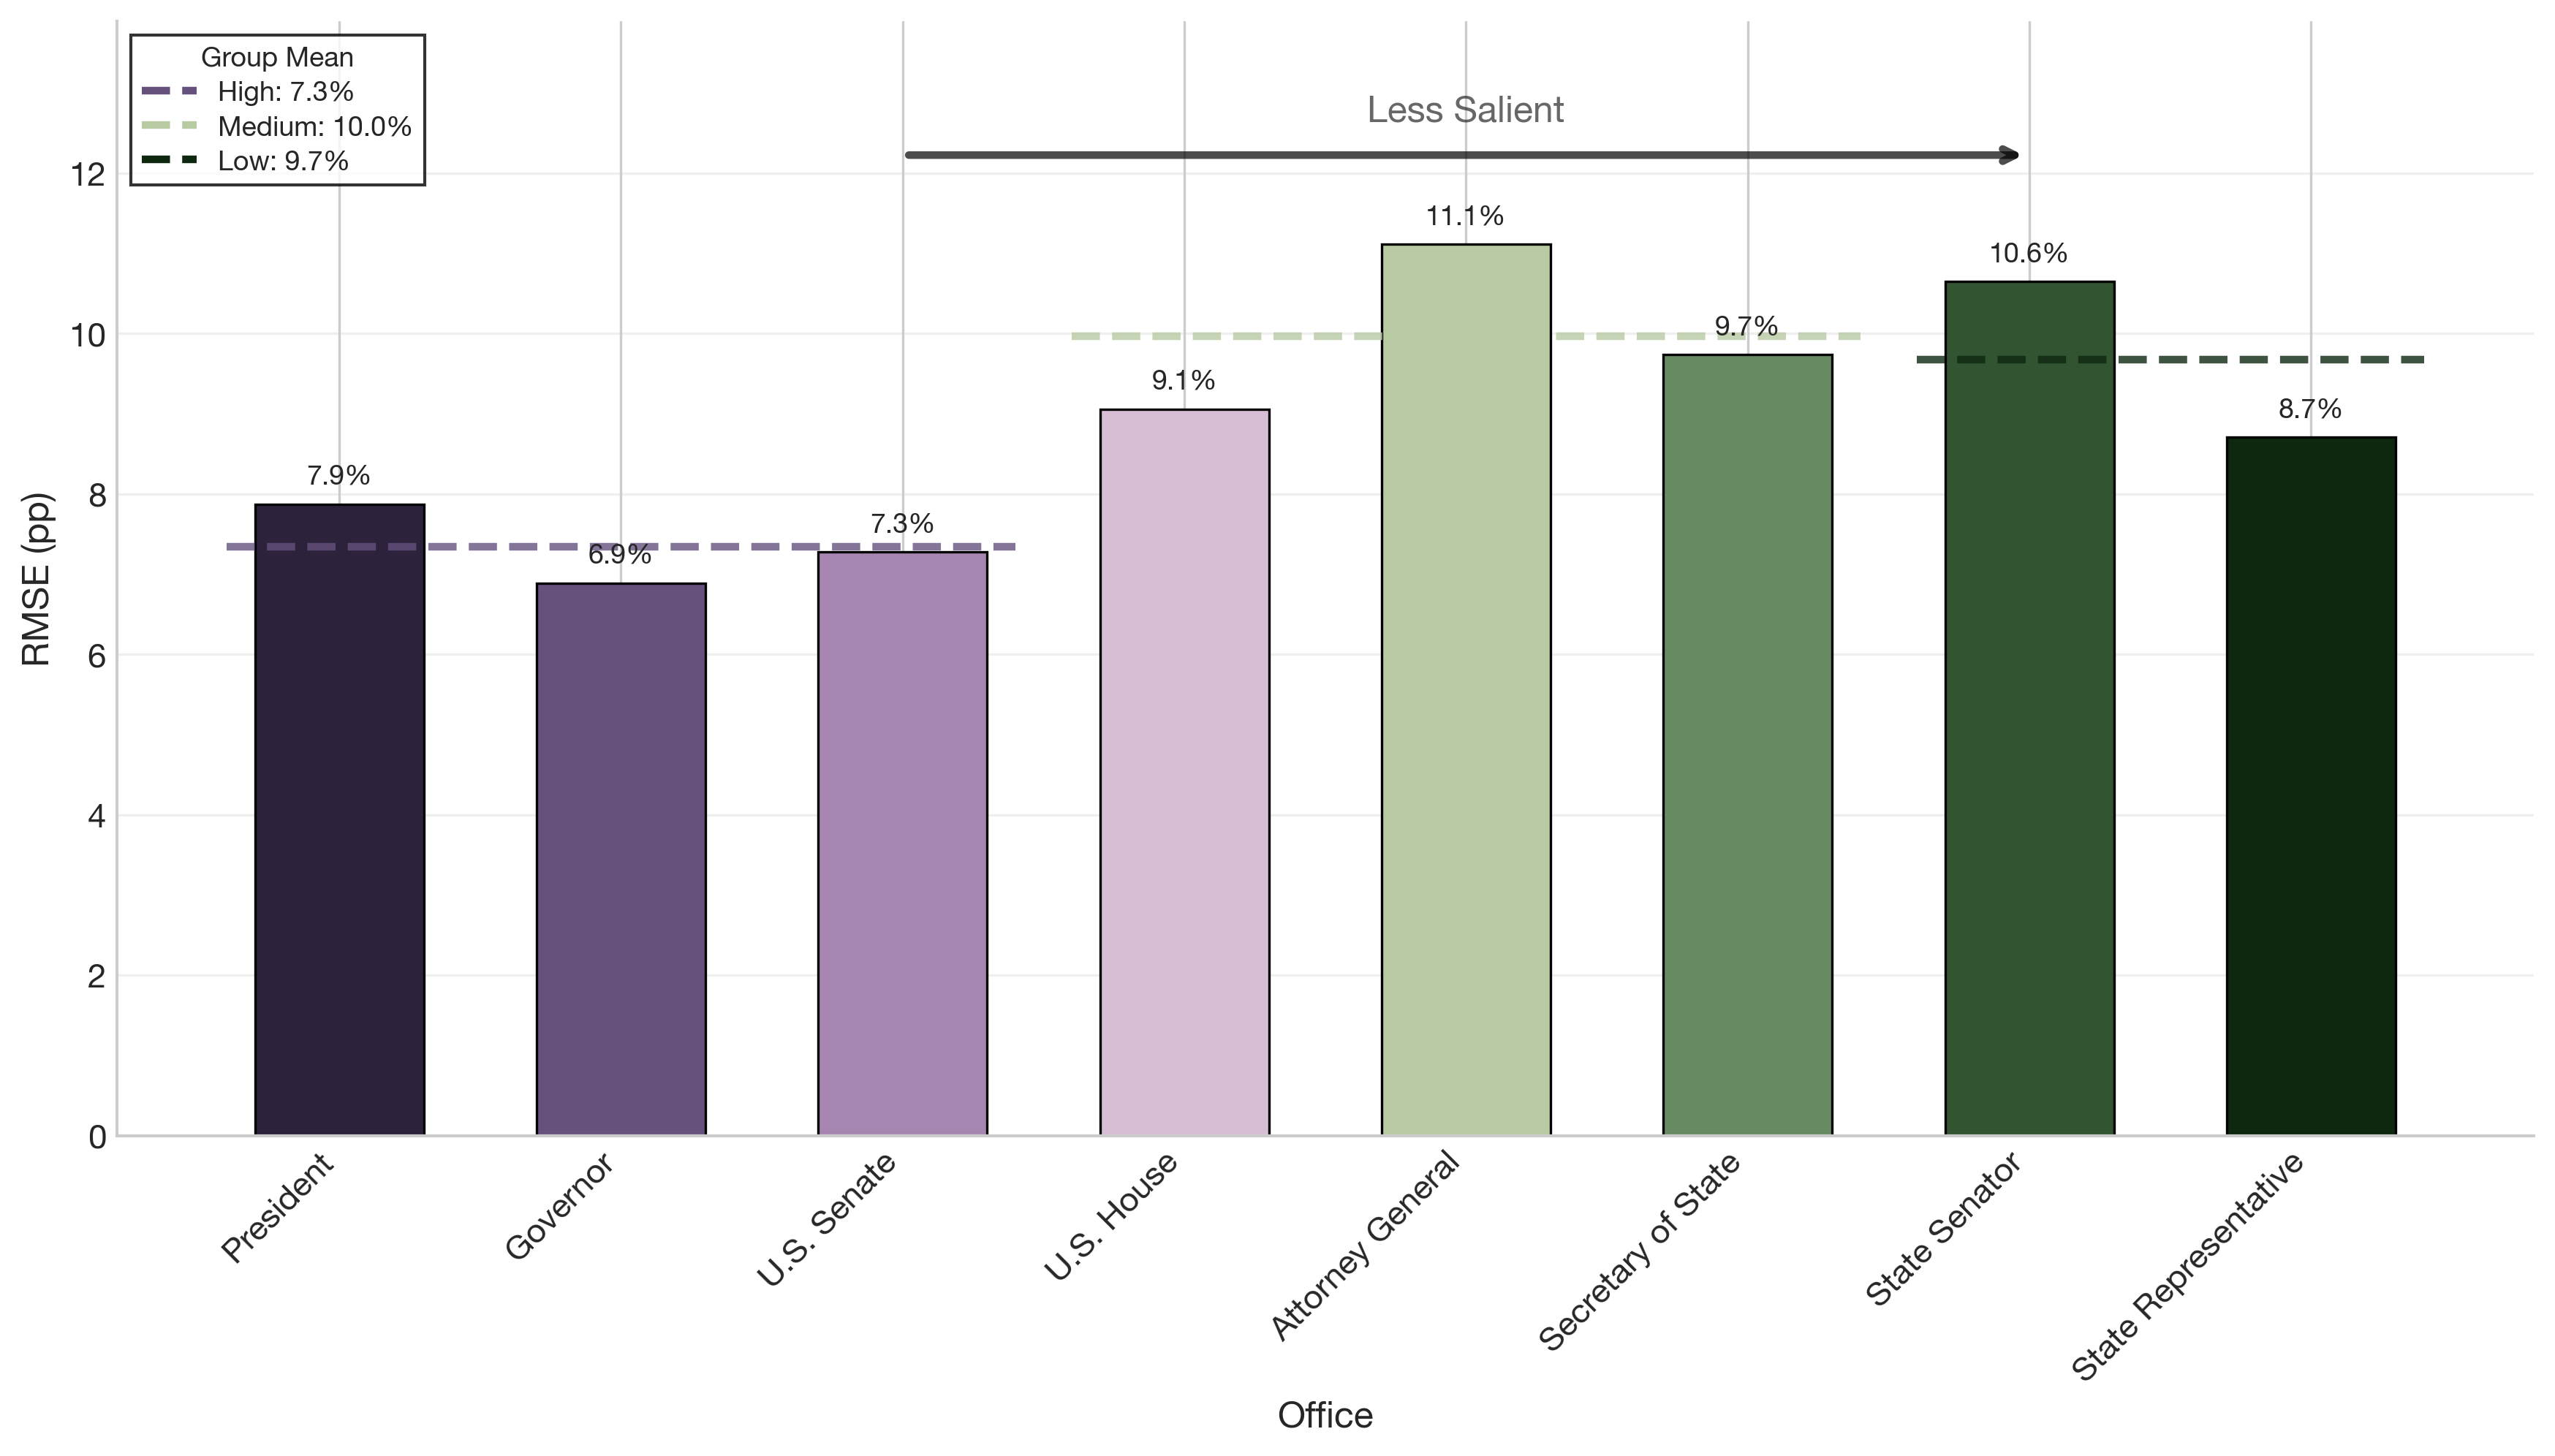
\includegraphics[width=\linewidth]{excluded_work/rmse_by_office_salience_party.png}
    \caption[RMSE by office salience]{RMSE by office salience. RMSE is computed across all party-level, unweighted observations for each office, pooled over the 2006--2022 waves rather than averaged across them, so a wave contributes in proportion to its number of observations. Dashed lines mark each salience group's mean, the simple average of its offices' pooled RMSEs.}
    \par\smallskip
    \noindent\begin{minipage}{\linewidth}\footnotesize\textit{Alt text:} Bar chart of error for eight offices ordered by salience, with dashed group averages: \SalienceHigh{} percentage points for high, \SalienceMedium{} for medium, and \SalienceLow{} for low salience offices.\end{minipage}
    \label{fig:rmse_by_office_salience_party}
\end{figure}


